\documentclass[12pt,a4paper]{article}
\usepackage[utf8]{inputenc}
\usepackage{amsmath}
\usepackage{amsfonts}
\usepackage{amssymb}
\usepackage{graphicx} 
\usepackage{color}
\usepackage{xcolor}
\usepackage{listings}
\usepackage{amsmath}
\usepackage{subfig}
\usepackage[]{algorithm2e}
\lstset{
language=C++,
basicstyle=\footnotesize\sffamily,
numbers=left,
numberstyle=\tiny,
breaklines=true,
frame=tb,
columns=fullflexible,
showstringspaces=false
}
\usepackage{caption}
\DeclareCaptionFont{white}{\color{white}}
\DeclareCaptionFormat{listing}

% This concludes the preamble
\title{technical report}
\begin{document}
\begin{titlepage}

\begin{center}
\LARGE Construction of analysis suitable mesh for the treatment of potential flow framework based on Spline surfaces

\end{center}
\begin{center}
 \Large \underline {Techical report}
\end{center}

\end{titlepage}



\tableofcontents
\pagebreak
\section{Domain overview}


\begin{center}
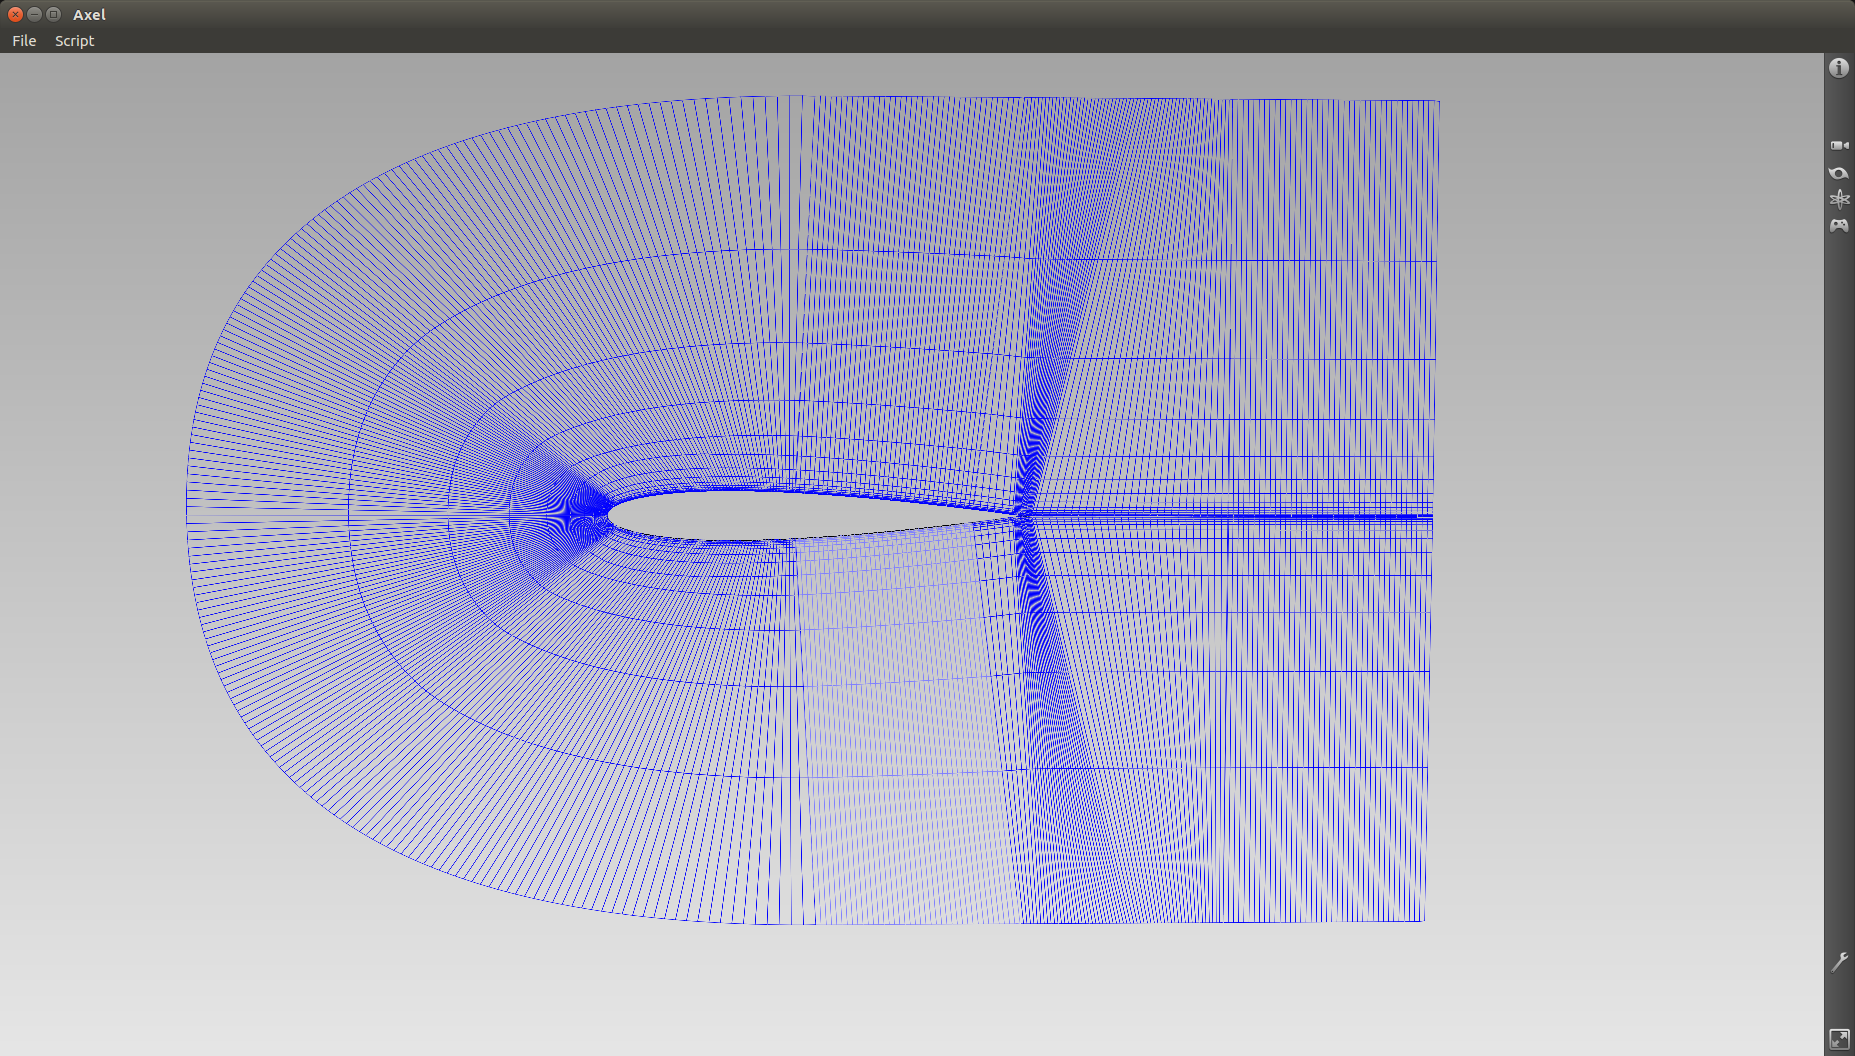
\includegraphics[scale=0.2]{SURFACES_AROUND_AIRFOIL.png} 
\end{center}


The goal of this work is to extract analysis suitable via parametrizing B-spline surfaces for the computation of potential flow problems around air foil.

Thus, for computational reasons we are interested in constructing a denser mesh (surfaces with denser knot line distribution by consequence) particularly int the following regions of the air foil:

\begin{itemize}
\item the trailing edge
\item the leading edge
\item Boundary around the  air foil

\end{itemize}


In what follows we give a description in the algorithms invoked for the completion of this goal.

\section{subdivision algorithm}

Let $s(t)\equiv s(u(t),v(t))$ and $k(\tau)\equiv k(u(\tau),v(\tau))$ denote the curve representing the foil and contour curve segment respectively.A subdivision algorithm(\textbf{\textit{Listing 1}}) located in  \textbf{get\_meshes.hpp} was put into place in order to obtain a manipulative distribution of  points $P_{i}(x(t_{i}),y(t_{i}))\in s(t)$ ,taking into consideration the curvature of the air foil and the euclidean distance of each point from the trailing edge .During the subdivision algorithm new point are selected applying the formula(\textbf{\textit{Listing 1,Line 28}}):

$$Q_{i}^{n}=\frac{P_{i-1}^{n-1}+P_{i}^{n-1}}{2}$$



where $P_{i-1}^{n-1},P_{i}^{n-1}\in s(t)$ and $Q_{i}^{n}$ is the mid point of the line segment formed by those two points .By projecting $Q_{i}^{n}$ to $s(t)$ we acquire the next point $P_{i}^{n}$(\textbf{\textit{Listing 1,Line 30}}) .


\begin{lstlisting}[label=some-code,caption=subdivision algorithm]
void get_meshes_contour(  axlAbstractCurveBSpline* axlcurve, axlAbstractCurveBSpline*  contour_curve,axlMesh* physical_mesh,axlMesh* parameter_mesh,const double points_on_line, double points_on_curve)
...
//subdivision algorithm for distribution of point along the
  airfoil
    std::vector<axlPoint> P;
    P.push_back(P0);
    P.push_back(P1);
    std::map<int,int> edge;
    edge[0]=1;
    int b,e;
    std::list<int> stack;
    stack.push_front(0);
    while(!stack.empty())
    {

        std::list<int>::iterator it=stack.begin();
        b=*it;
        stack.pop_front();
        e=edge[b];
        axlPoint P_b=P.at(b);
        axlPoint  P_e=P.at(e);

        double   u_b=dst.nearestCurveParameter(P_b.x(),P_b.y(),P_b.z(),i);
        double  u_e=dst.nearestCurveParameter(P_e.x(),P_e.y(),P_e.z(),i);

        if (axlPoint::distance(P_b,P_e)*alt_distance_factor(P_b,P_e)*curvature_factor(axlcurve,u_b,u_e)>(1/points_on_curve))
        {
            axlPoint P_middle_on_line=(P.at(b)+P.at(e))/2;
            double u_projected=dst.nearestCurveParameter(P_middle_on_line.x(),P_middle_on_line.y(),P_middle_on_line.z(),i);
            axlPoint P_middle_projected=axlcurve->eval(u_projected);
            P.push_back(P_middle_projected);
            int n=P.size()-1;
            edge[b]=n;
            edge[n]=e;
            stack.push_back(b);
            stack.push_back(n);
        }
           
  ....    }
\end{lstlisting}


\vspace{5pt}
The subdivision algorithm takes into consideration the following criteria(\textbf{\textit{Listing 1,Line 26}}): 

\begin{frame}

\begin{minipage}{1\linewidth}
\begin{center}

\begin{algorithm}[H]


\eIf{\small
$(d(P_{i-1}^{n-1},P_{i}^{n-1})
*f_{dist}(d(P_{i-1}^{n-1},A),d(P_{i}^{n-1},A))
*g_{curv}(P_{i-1}^{n-1},P_{i}^{n-1})\geq \frac{1}{N_{0}})$
}{
proceed Subdivision\;
}{
Stop\;
}
\end{algorithm}

\end{center}
\end{minipage}

\end{frame}




\vspace{5pt}
$d(P_{i-1}^{n-1},P_{i}^{n-1})$ denotes the euclidean distance between  these points,\\$f_{dist}(d(P_{i-1}^{n-1},A),d(P_{i}^{n-1},A))$ is a function taking into account the euclidean distance $d(P_{i-1}^{n-1},A)$ and $d(P_{i-1}^{n-1},A)$ , $A \in s(t)$ being the trailing edge point of the air foil and last $g_{curv}(P_{i-1}^{n-1},P_{i}^{n-1}) $ a function taking into account the curvature of the points.${N_{0}}$ denotes the user input  total number of points on the air foil.






 


 
 \subsection{Distance from trailing edge}
 
the $f_{dist}$ function located in \textbf{alt\_distance.hpp}  as mentioned above takes into account the euclidean distance of the points  $P_{i-1}^{n-1},P_{i}^{n-1}$ from the trailing edge $A$ the \textit{point\_{radius}} parameter(\textbf{\textit{Listing 2,Line 9}}) adjusts the radius of the effect around the trailing edge and is defined as follows:
 
 
$$ f_{dist}=\begin{cases} 1 , if \:  \Vert P_{i-1}^{n-1}A \Vert + \Vert P_{i}^{n-1}A \Vert >point\_radius \\ b-(\frac{b-1}{point\_radius})(\Vert P_{i-1}^{n-1}A \Vert + \Vert P_{i}^{n-1}A \Vert) , \;else \end{cases}$$ 
 
 

\begin{figure}[h]
  \centering
  \subfloat[point\_{radius}=0.03]{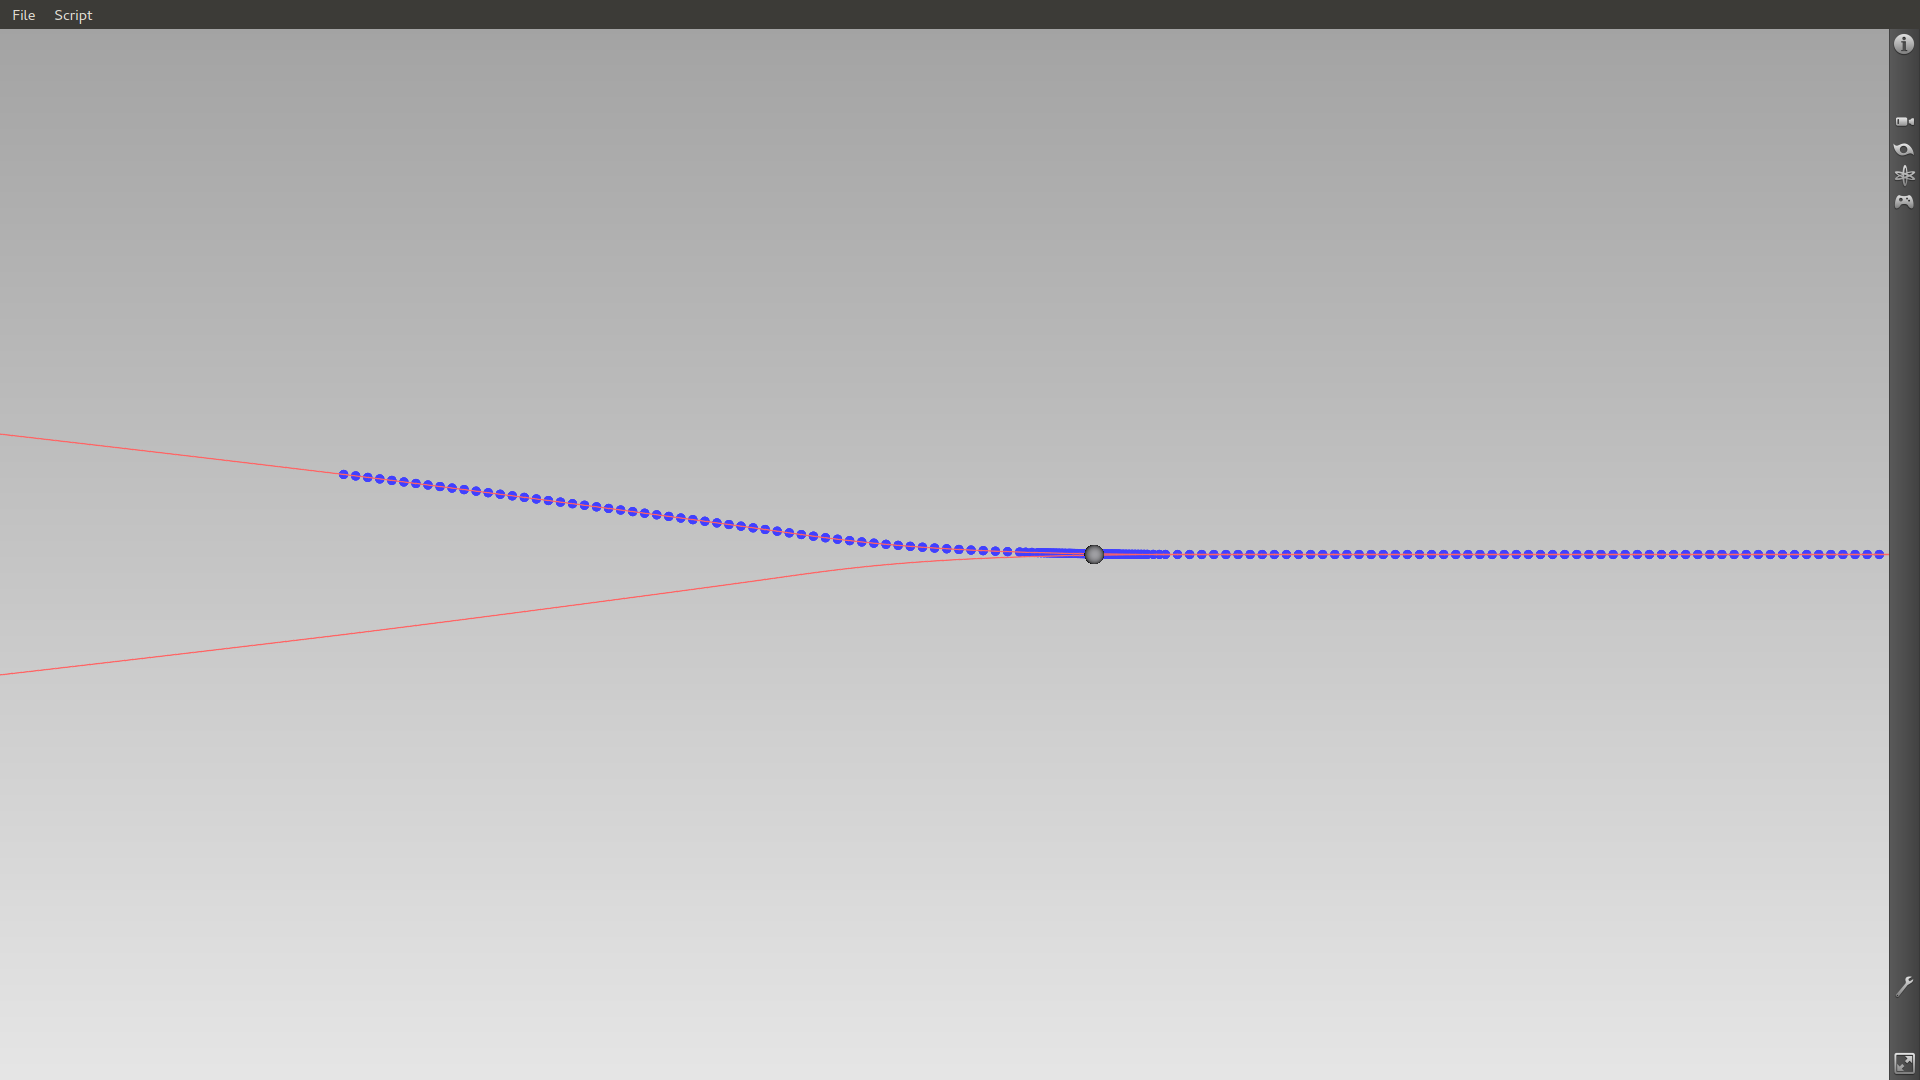
\includegraphics[width=0.5\textwidth]{PICTURES2/Distance_effect_003.png}\label{fig:f1}}
  \hfill
  \subfloat[point\_{radius}=0.12]{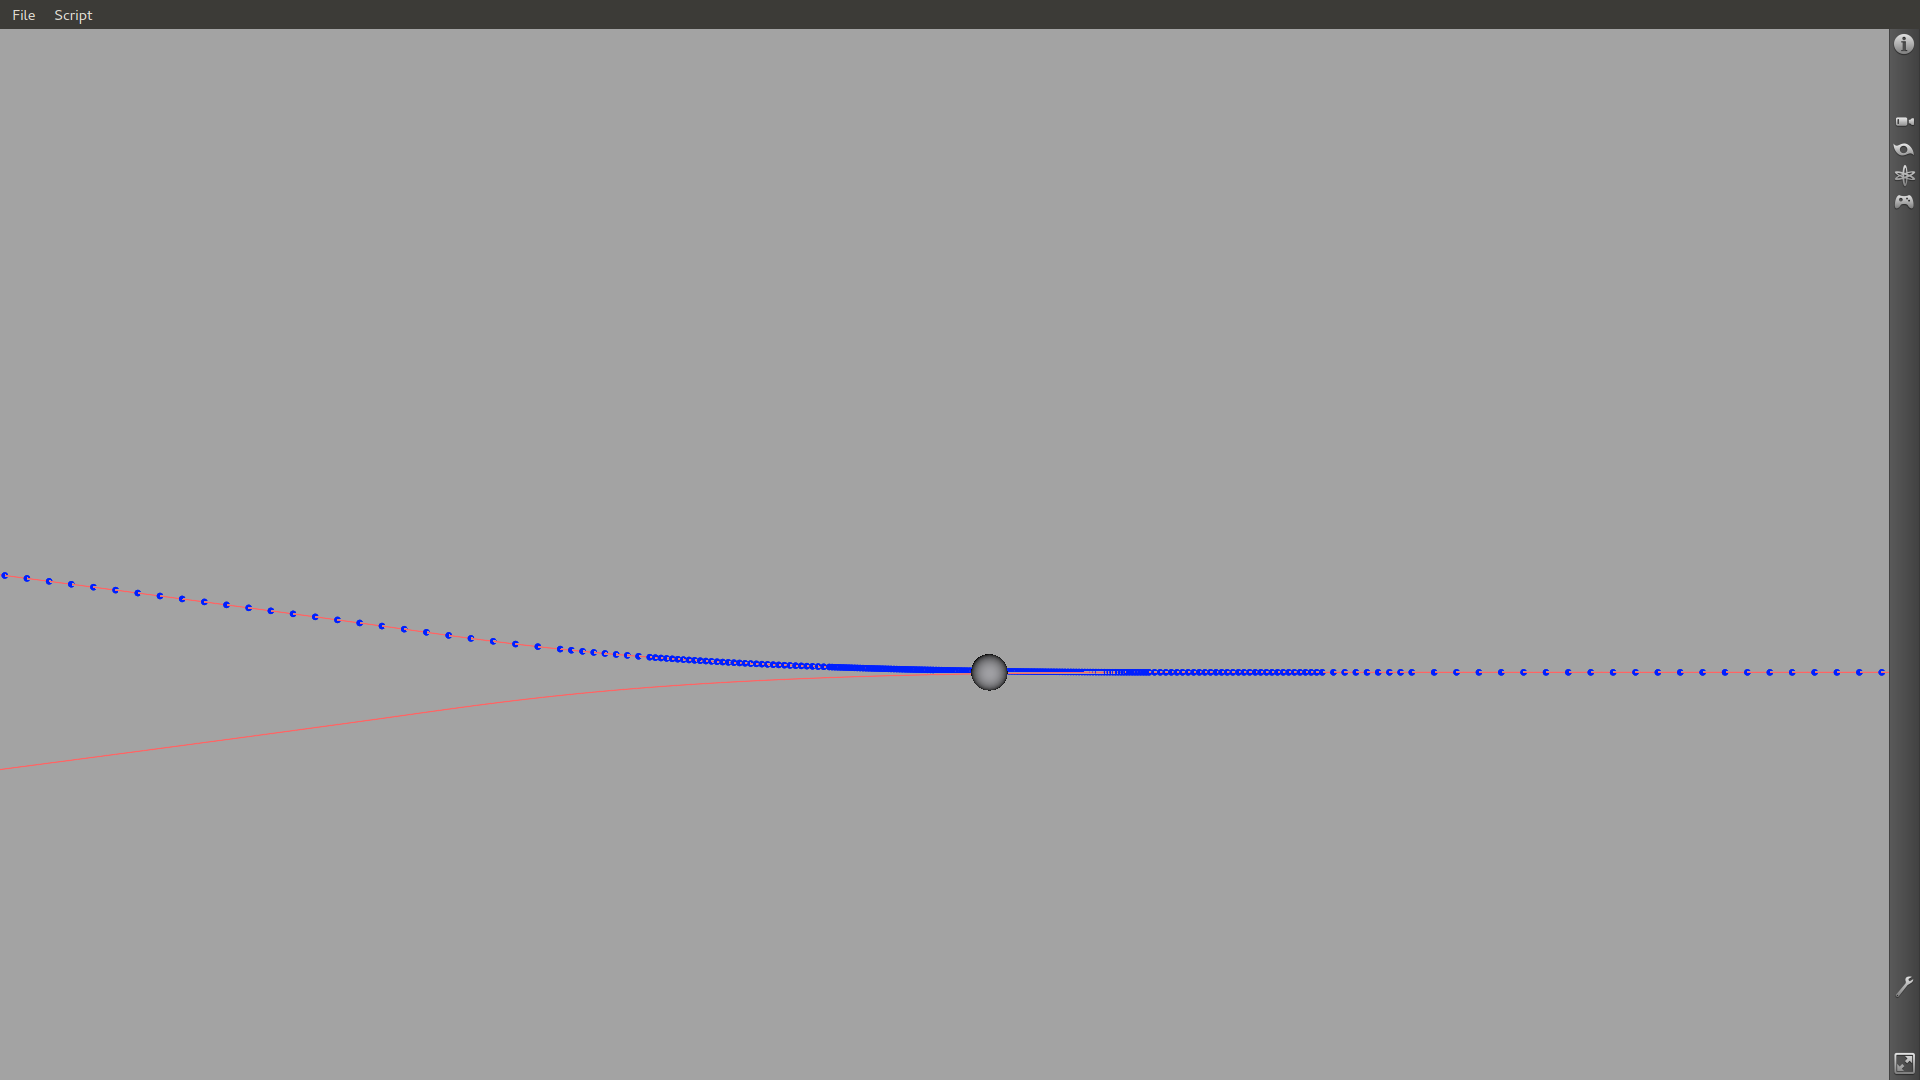
\includegraphics[width=0.5\textwidth]{PICTURES2/Distance_effect_056.png}\label{fig:f2}}
  \caption{Distribution of points after distance from the trailing edge factor for different values of \textit{point\_{radius}} parameter }
\end{figure}


\pagebreak
\begin{lstlisting}[label=some-code,caption=distance from trailing edge factor]
double alt_distance_factor(const axlPoint& P1,const axlPoint& P2)
{  axlPoint trailing_edge(1,0,0);

    double distance_P1=axlPoint::distance(P1,trailing_edge);
    double distance_P2=axlPoint::distance(P2,trailing_edge);
    double sum_of_distances=distance_P1+distance_P2;
    double distance_factor;

    double point_radius=0.1;
    double b=10;


    if (sum_of_distances>point_radius)
    {
        distance_factor=1;
    }
    else
    {
        distance_factor=b-((b-1)/point_radius)*sum_of_distances;
    }

    return distance_factor;
}
\end{lstlisting}

 

 
\subsection{curvature factor}

the $g_{curv}$ function takes into account the curvature of $P_{i-1}^{n-1},P_{i}^{n-1}$ , the \textit{region\_{effect}}(\textbf{\textit{Listing 3,Line 12}}) parameter adjusts the sensibility of the effect around the air foil and is defined as follows(\textbf{\textit{Listing 3,Lines 18-27}}):\\
 

$$ g_{curv}=\begin{cases} b-(\frac{b-1}{region})\left(  \frac{1}{curv(P_{i-1}^{n-1})}+\frac{1}{curv(P_{i-1}^{n})}\right) ,if \frac{1}{curv(P_{i-1}^{n-1})}+\frac{1}{curv(P_{i-1}^{n})} >region\_{effect} \\ 1, else \end{cases} $$


where $$curv(P(u(t),v(t)))=\frac{u(t)'v(t)''-v(t)'u(t)''}{(u(t)'^2+v(t)'^2)^{3/2}}$$

denotes the curvature of the point .
 
 \begin{lstlisting}[label=some-code,caption=curvature factor]
double curvature_factor(axlAbstractCurveBSpline* axlcurve,double u_a,double u_b)
{   
    double curv_a=curvature( axlcurve ,u_a);
    double curv_b=curvature(axlcurve,u_b);
    double radius_a=1/curv_a;
    double radius_b=1/curv_b;
 
    double sum_of_curvatures=radius_a+radius_b;


    double b=10;
    double region_effect=0.2;
    double curve_factor;




    if (sum_of_curvatures<region_effect)
    {
        curve_factor=(b-((b-1)/region_effect)*sum_of_curvatures);
    }
    else
    {
        curve_factor=1;
    }

    return curve_factor;

}


\end{lstlisting}

 

\begin{figure}[h]
  \centering
  \subfloat[curvature\_{effect}=0.2]{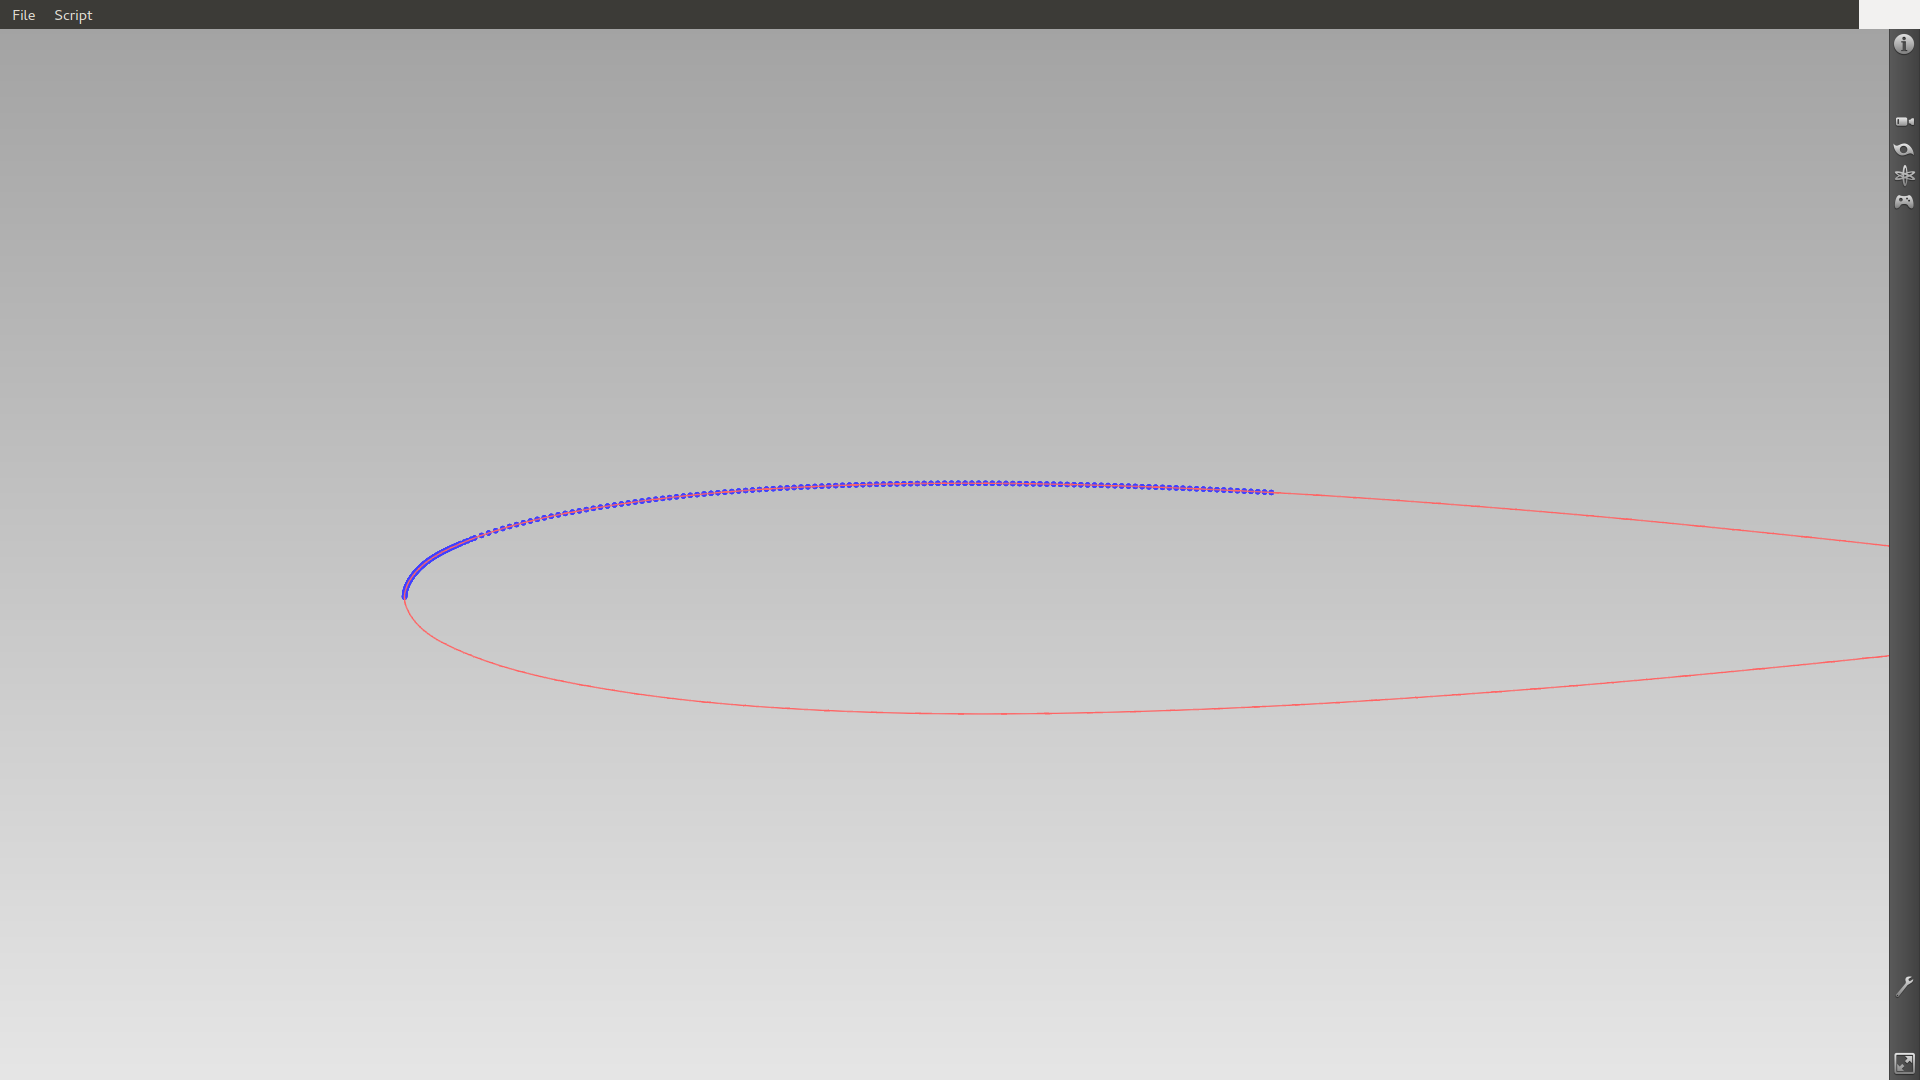
\includegraphics[width=0.5\textwidth]{PICTURES2/curvature_effect_02.png}\label{fig:f1}}
  \hfill
  \subfloat[curvature\_{effect}=0.7]{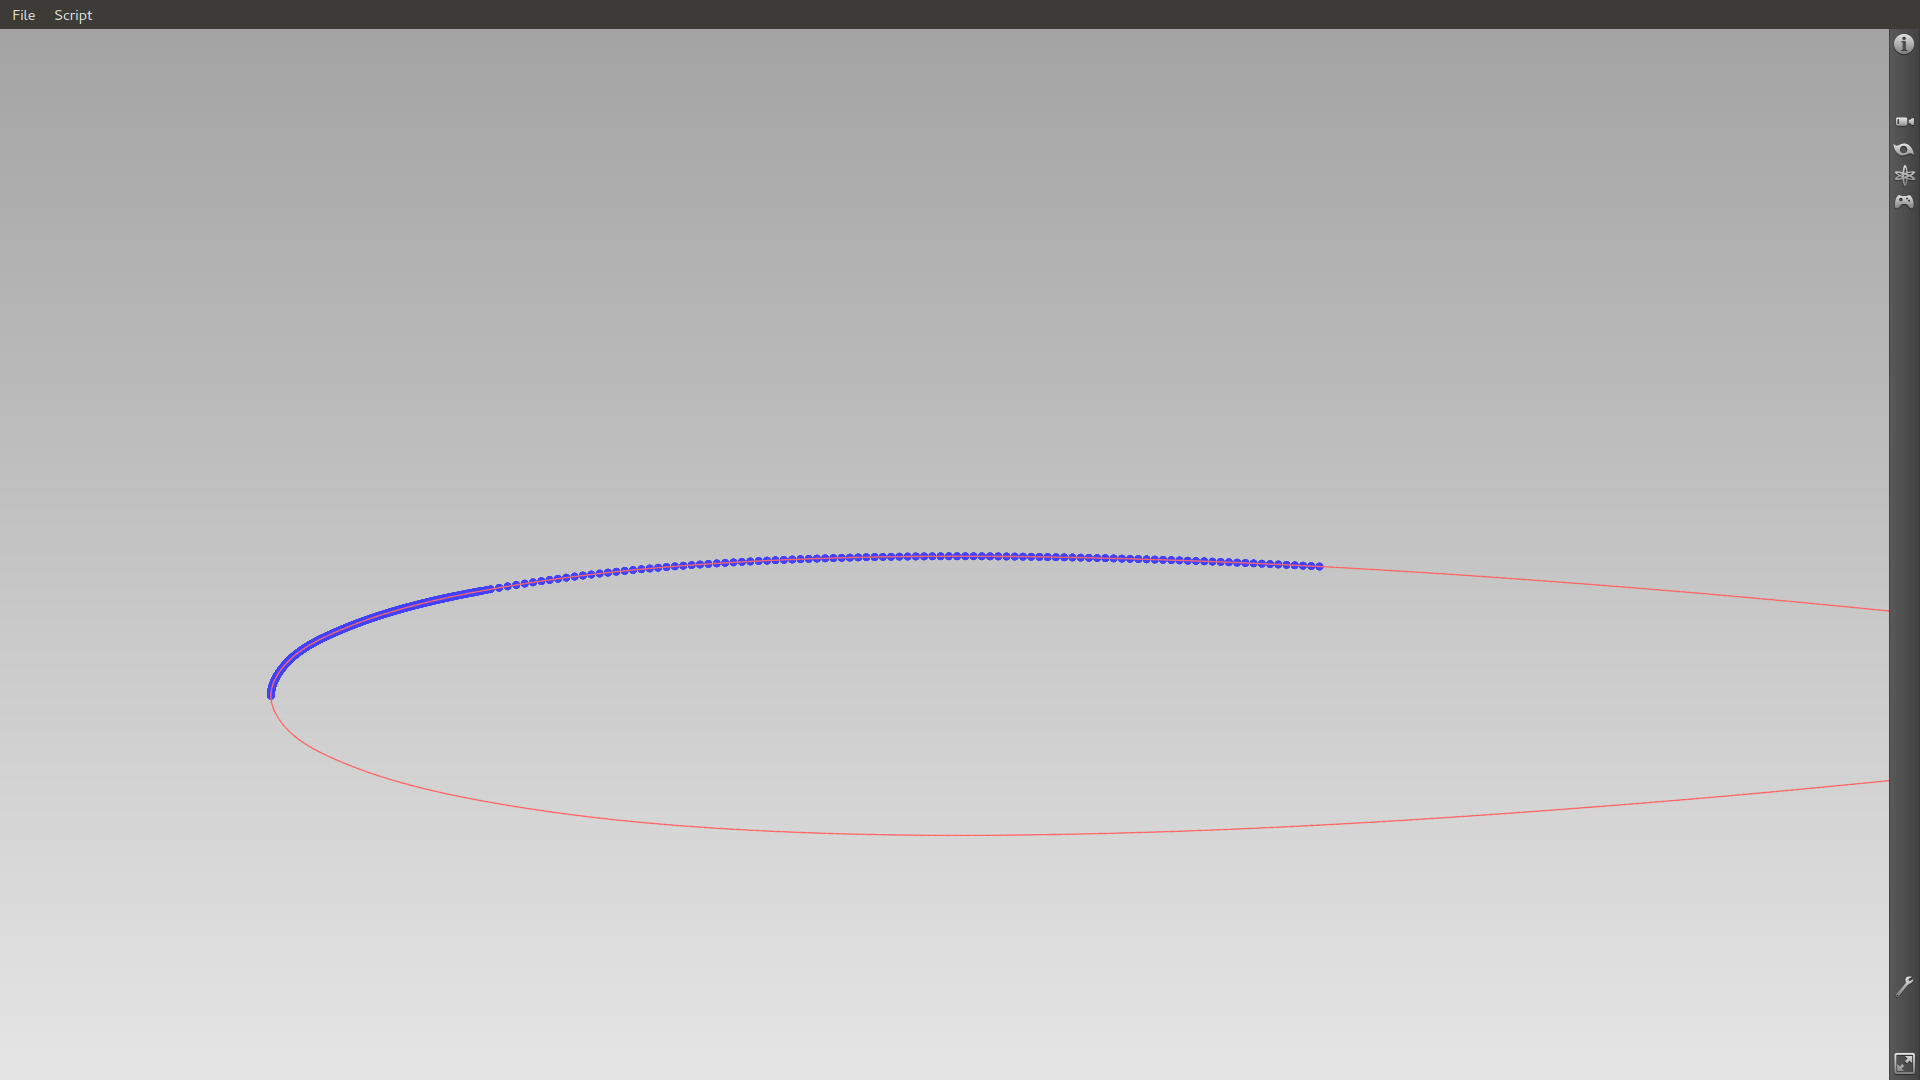
\includegraphics[width=0.5\textwidth]{PICTURES2/curvature_effect_07.png}\label{fig:f2}}
  \caption{Distribution of points after distance from the trailing edge factor for different values of \textit{region\_{effect}} parameter}
\end{figure}


\subsection{Distribution of points selected for the construction of the physical mesh }
Now that we assembled $P_{i} \in s(t)$ ,$i\in \lbrace 0,1,...N \rbrace $ we proceed by constructing the physical mesh of points. By collecting  $X_{i} \in k(\tau)$ in uniform fashion we then choose points  $Q_{ij}$ along the line segments $P_{i}X_{i}$ .The selection takes place in \textbf{get\_meshes.hpp} , \textbf{get\_meshes\_contour(...)} function after the subdivision algorithm.
\\
If  $M$ is the  input of points on line  variable of the user then(\textbf{\textit{Listing 4,25}}) :


$$Q_{ij}=P_{i}+(X_{i}-P_{i})*l_{0}*\frac{a^{j+1}-1}{a-1} , where \; i\in \lbrace 0,1,...,N \rbrace  \; and\; j\in \lbrace 0,1,..M\rbrace
$$

where $l_{0}=\frac{a-1}{a^{M}-1}$ and $a$ is a scaling factor.



\begin{figure}[h]
  \centering
  \subfloat[a=1.1]{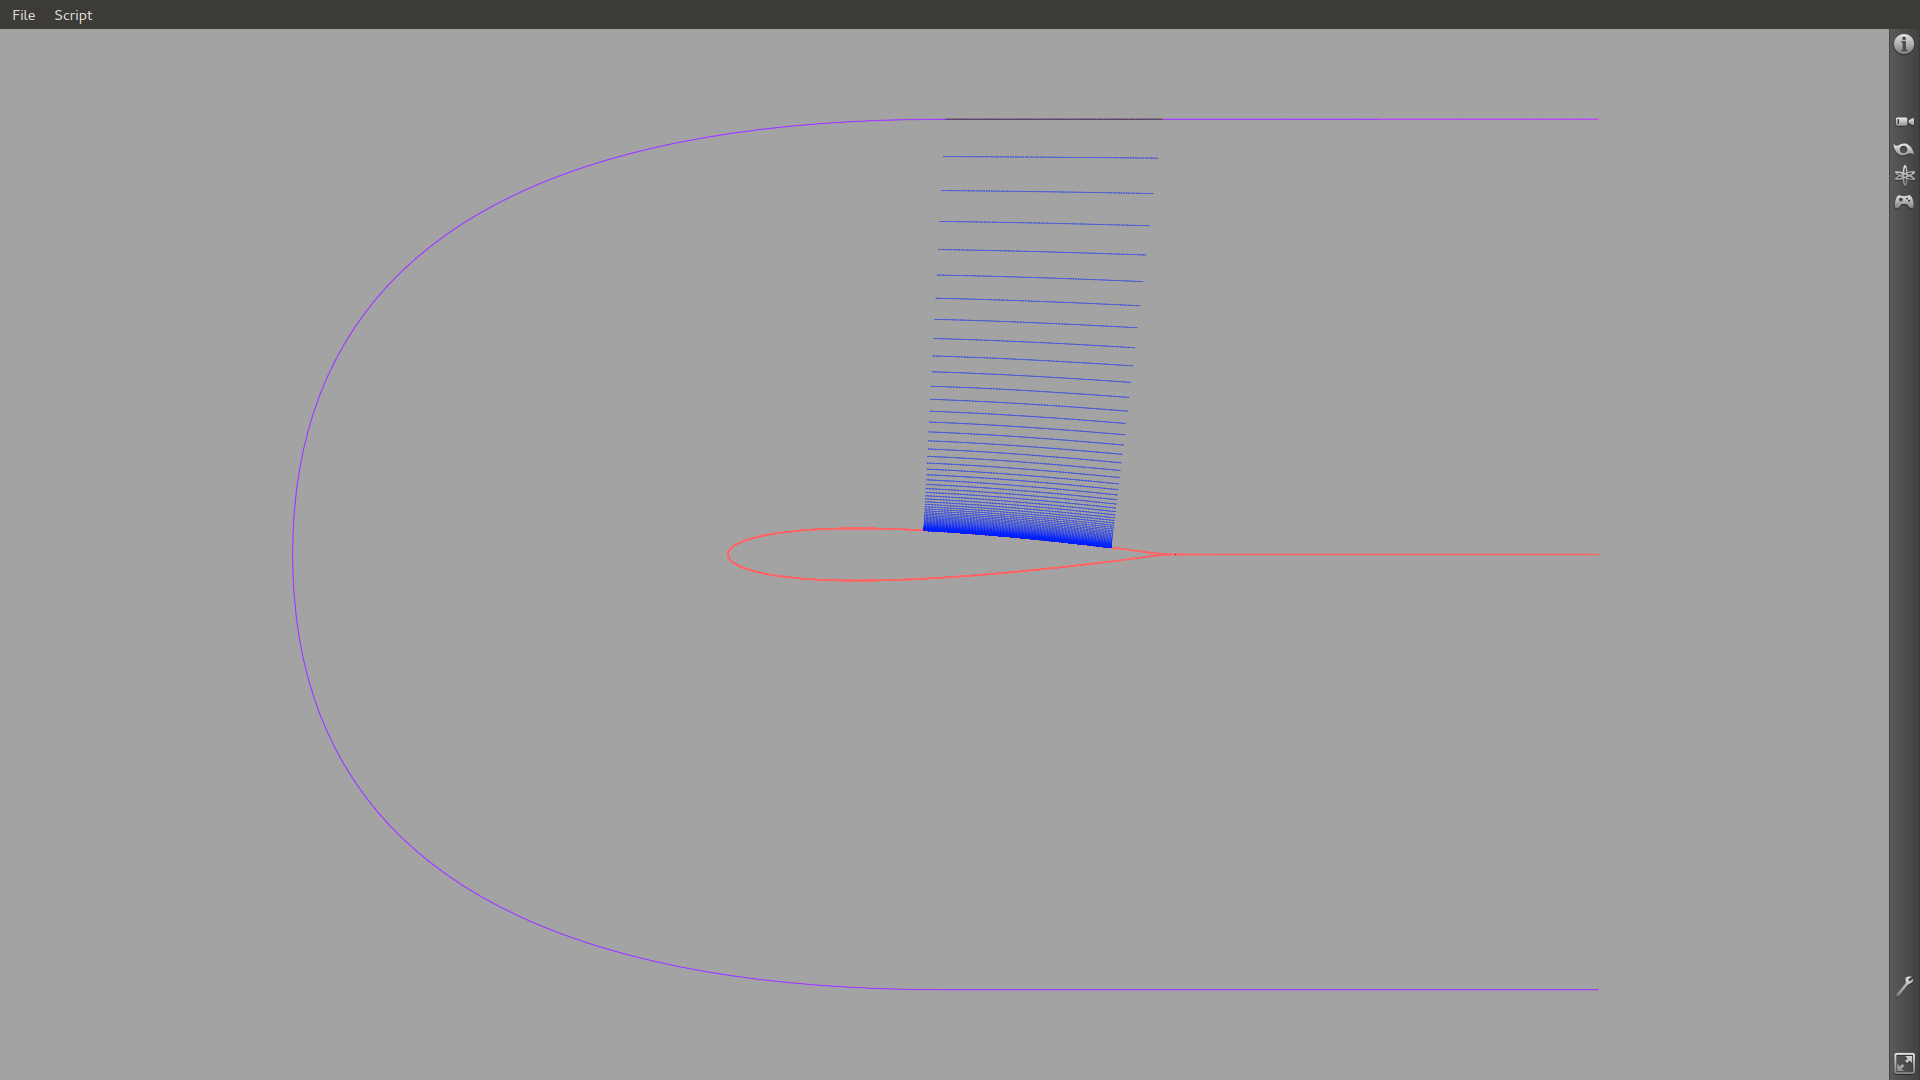
\includegraphics[width=0.5\textwidth]{PICTURES2/scaling_factor_11.png}\label{fig:f1}}
  \hfill
  \subfloat[a=1.7]{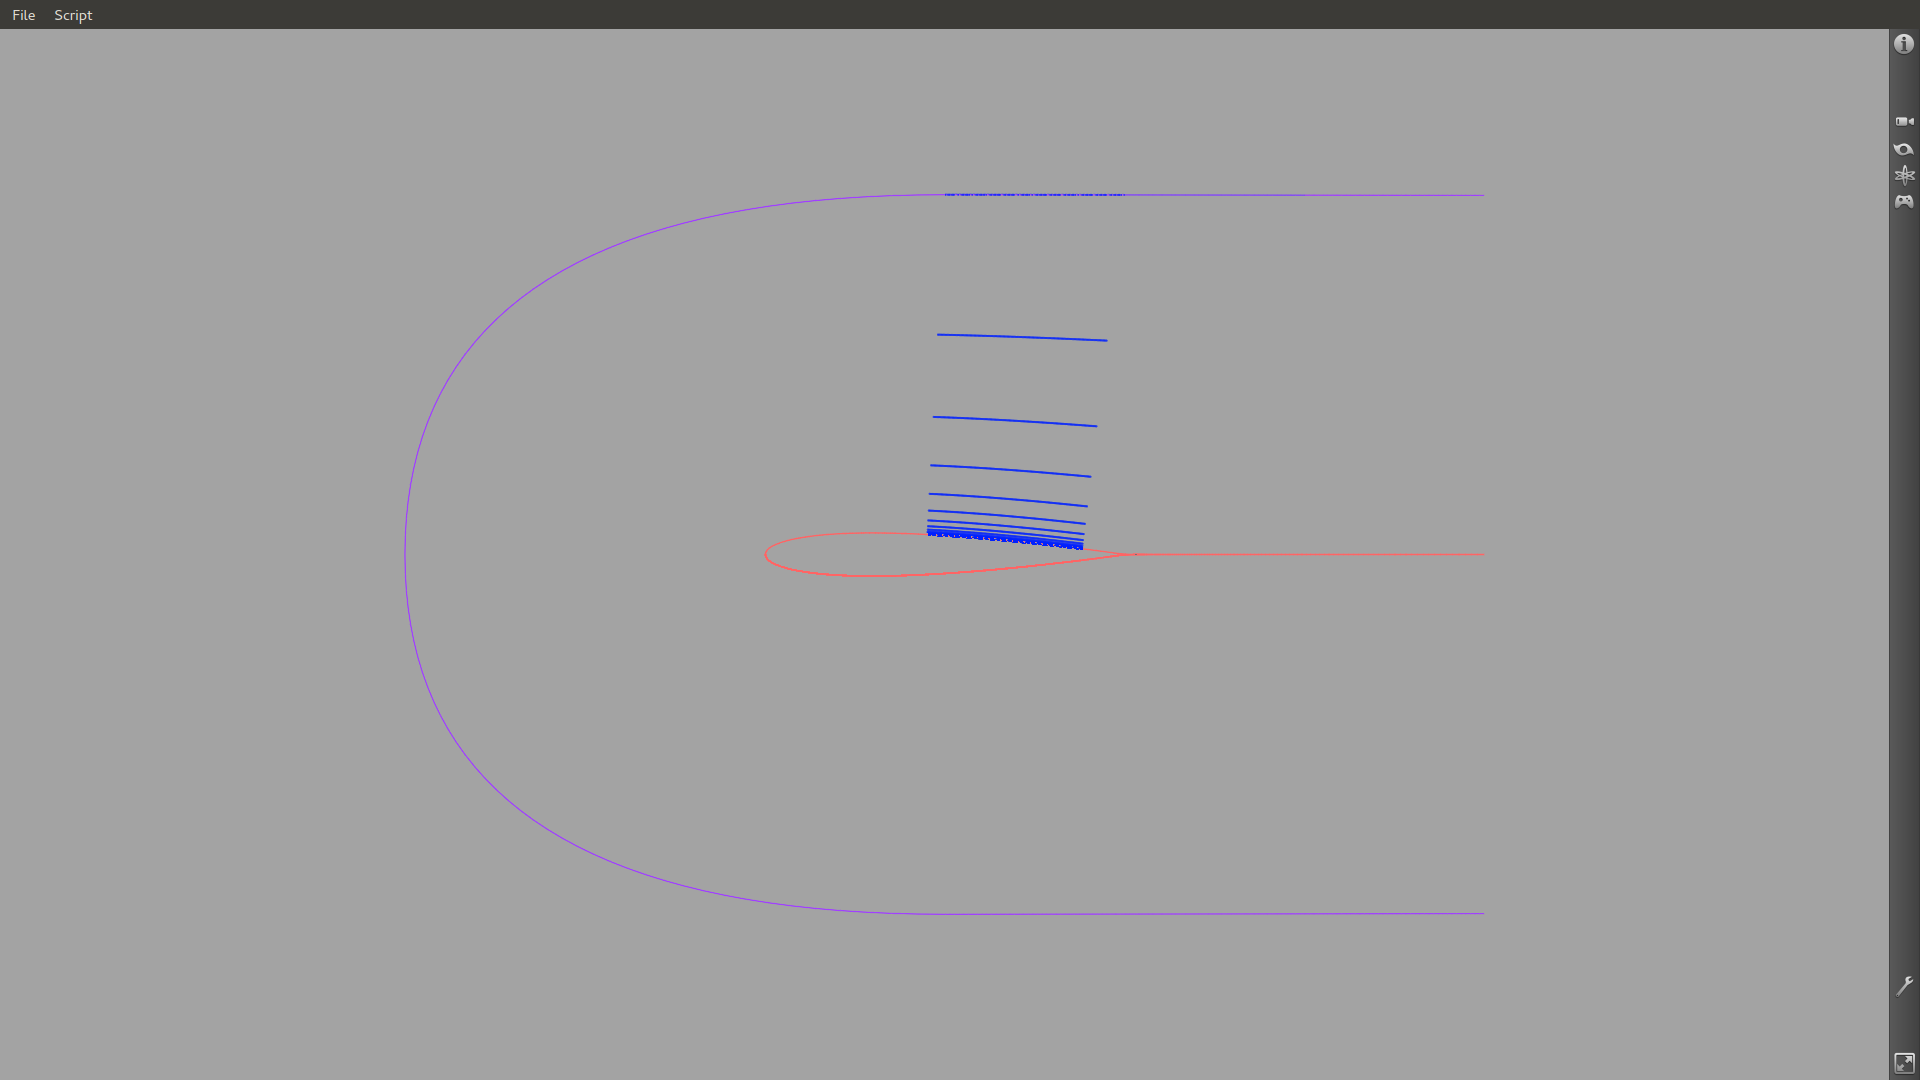
\includegraphics[width=0.5\textwidth]{PICTURES2/Scaling_factor_17.png}\label{fig:f2}}
  \caption{The effect of scaling factor $a$ on selection of points}
\end{figure}





\begin{lstlisting}[label=some-code,caption=Creation of the physical mesh of points]
void get_meshes_contour(  axlAbstractCurveBSpline* axlcurve, axlAbstractCurveBSpline*  contour_curve,axlMesh* physical_mesh,axlMesh* parameter_mesh,const double points_on_line, double points_on_curve)
{...   
   //initialization of selection of  points v-direction for each of the subdivision points
    step=0;
    std::vector<double> step_vector;
    for(int i=0;i<=points_on_line;i++)


    {
        step_vector.push_back(step);
    }

    for (int i=0;i<points_on_curve;i++)
    {
        axlPoint Pi=P.at(i);
        axlPoint X=contour_curve->eval(step);
        physical_mesh->push_back_vertex(P.at(i));

        double distance_PiX=axlPoint::distance(Pi,X);
        distances_d.push_back(dst.distance(Pi.x(),Pi.y(),Pi.z()));
        distances_l.push_back(0);

        for(double j=1;j<=points_on_line;n++)

        {   axlPoint Q=Pi+(X-Pi)*(l0*(((pow(a,n+1))-1)/(a-1)));
            physical_mesh->push_back_vertex(Q);


            double distance_QPi=axlPoint::distance(Q,Pi);
            double distance_l=distance_QPi/distance_PiX;
            double distance_d=dst.distance(Q.x(),Q.y(),Q.z());

            if (j==points_on_line)
            {
                distances_l.push_back(1);
            }
            else
            {

                distances_l.push_back(distance_l);}
            distances_d.push_back(distance_d);
        }

        step+=1/(points_on_curve);

        for(int i=0;i<=points_on_line;i++)


        {
            step_vector.push_back(step);
        }

  ...  }

\end{lstlisting}


\subsection{Parametric Domain}


In \textbf{{get\_meshes.hpp}},\textbf{get\_meshes\_contour(...)} we then proceed by constructing the parameter domain $\widehat{\Omega}$ which will be mapped to the physical domain $\Omega$ via the fitting process.Coordinates $(u_{i},v_{i})$ are equal to:



$$u_{i}=i/N$$ 
where $i\in \left\lbrace 0,1,2,..M \right\rbrace  $,M being the number on the points on curve determined the subdivision algorithm.and $$v_{i}=log(v_{i_{0}}+b_1)-\frac{log(b_1)}{log(a_1)}$$

which is a result of the logarithmic transformation of(\textbf{\textit{Listing 5,Line 21}}): $$v_{i_{0}}=\delta\Vert Q_{ij} P_{i}\Vert+(1-\delta)(\frac{\Vert Q_{ij} P_{i}\Vert}{\Vert  P_{i}X_{i}\Vert})$$ and

$$\delta =\begin{cases}0, if  \Vert Q_{ij} P_{i}\Vert <d_{0} \\ 2d_{0}-\Vert Q_{ij} P_{i}\Vert, if \Vert Q_{ij} P_{i}\Vert <2d_{0}\\0 , else
\end{cases}$$

 
 where $a_1=a^{M}-1$  and $b_1=\frac{1}{a-1}$ and $M$ is total of points along the line segments $P_{i}X_{i}$.Thus taking into account the barycentric position of $Q_{ij}$ along the line segment $P_{i}X_{i}$ when we're closer to the air foil($d_0$ affecting the criteria).


With the parametric and physical mesh in place we now proceed to the fitting process located in \textbf{get\_surface.hpp}.
The parametric coordinates are then mapped to the physical domain via the function $S(u,v)=\sum_{i}\sum_{j} R_{ij}(u,v)d_{ij}$ ,where $d_{ij}$ are the control points determined by the fitting algorithm(\textbf{\textit{Listing 6,Line 26}}).



 \begin{lstlisting}[label=some-code,caption=Parametric coordinates]
void get_meshes_contour(  axlAbstractCurveBSpline* axlcurve, axlAbstractCurveBSpline*  contour_curve,axlMesh* physical_mesh,axlMesh* parameter_mesh,const double points_on_line, double points_on_curve)
{... 

//Creating parameter mesh
    double delta;
    std::vector <double> v;
    for(int j=0;j<distances_d.size();j++) {
        if(distances_d.at(j)<=d0)
        {
            delta=1;
        }
        else if( (distances_d.at(j)<=2*d0) )
        {
            delta=(((2*d0)-distances_d.at(j)));

        }else
        {
            delta=0;
        }
        double v0=((delta)*distances_d.at(j))+((1-delta)*distances_l.at(j));
        v0=(log(v0+b1)-log(b1))/log(a1);
        v.push_back(v0);

        parameter_mesh->push_back_vertex(step_vector.at(j),v.at(j),0);

    }
    
   ... }

\end{lstlisting}





\begin{figure}[h]
  \centering
  \subfloat[]{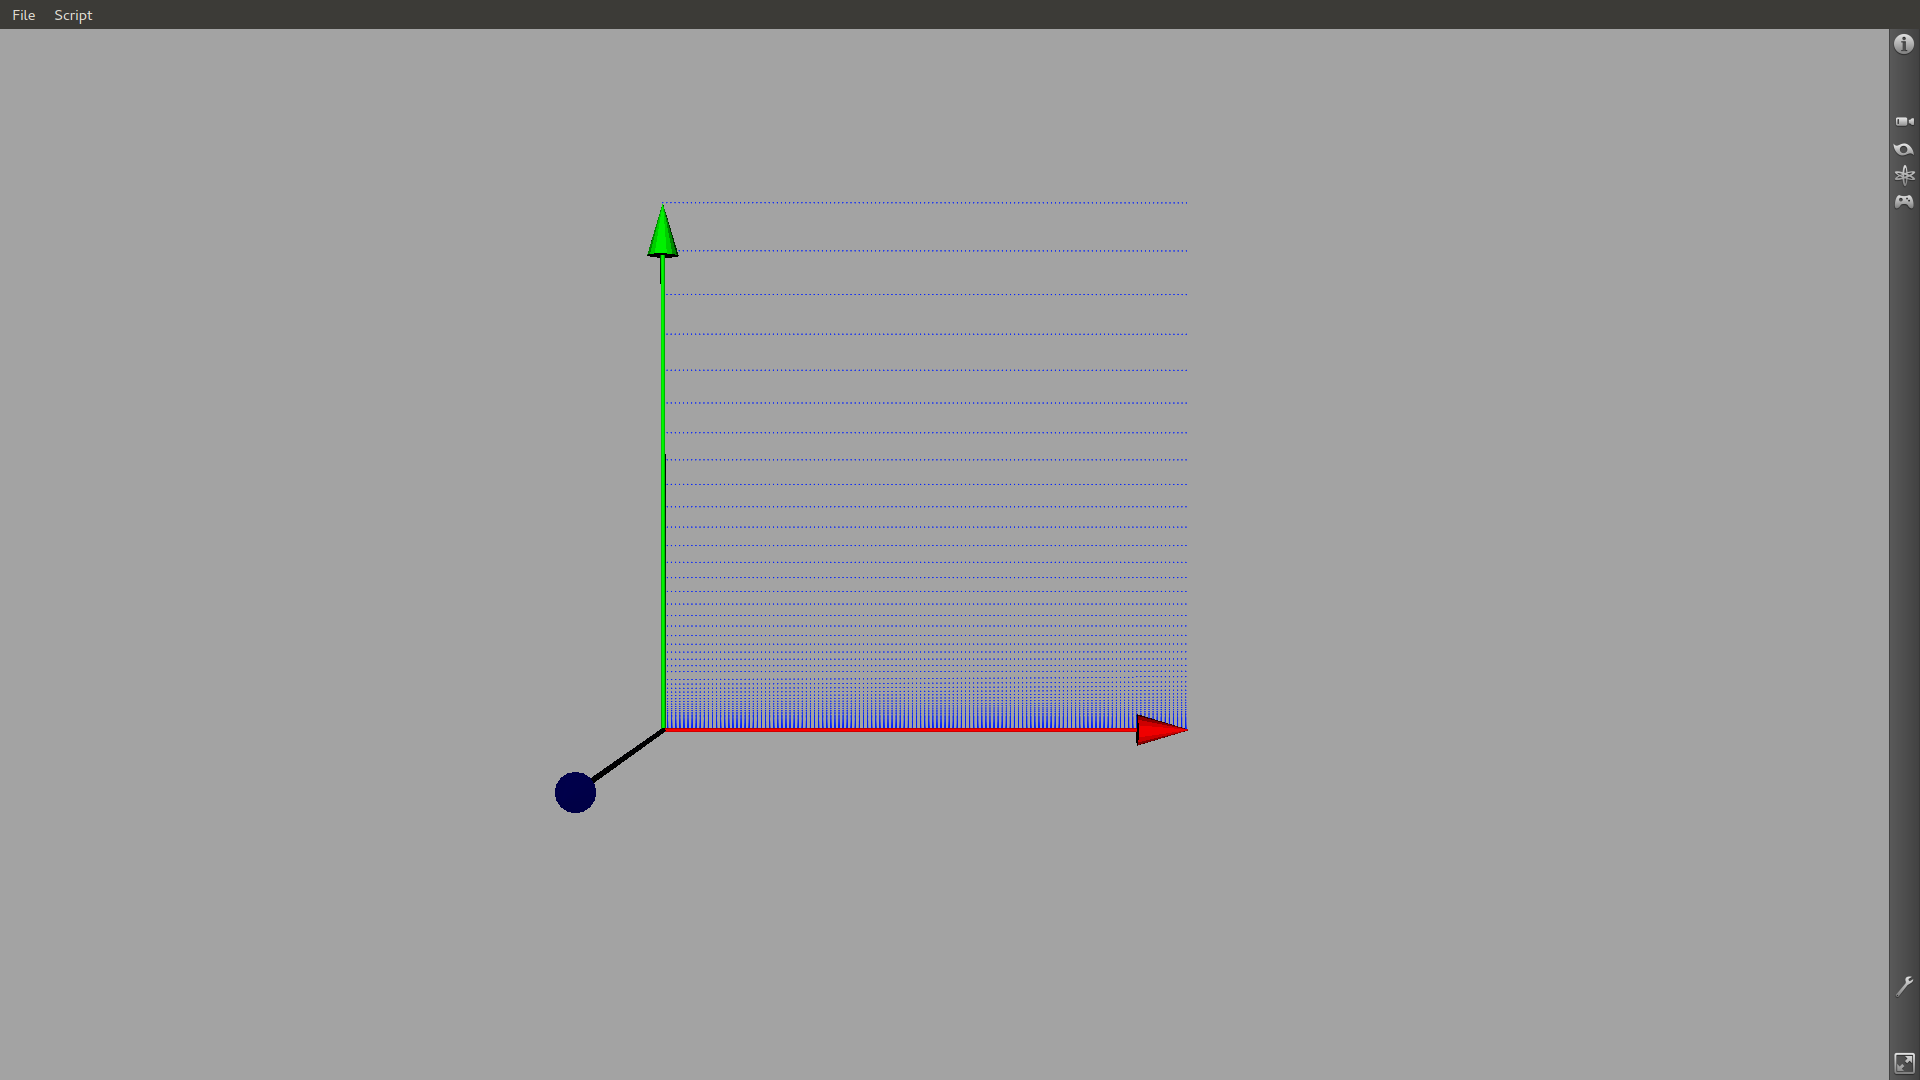
\includegraphics[width=0.5\textwidth]{PICTURES2/parameter_non_logarithmic.png}\label{fig:f1}}
  \hfill
  \subfloat[]{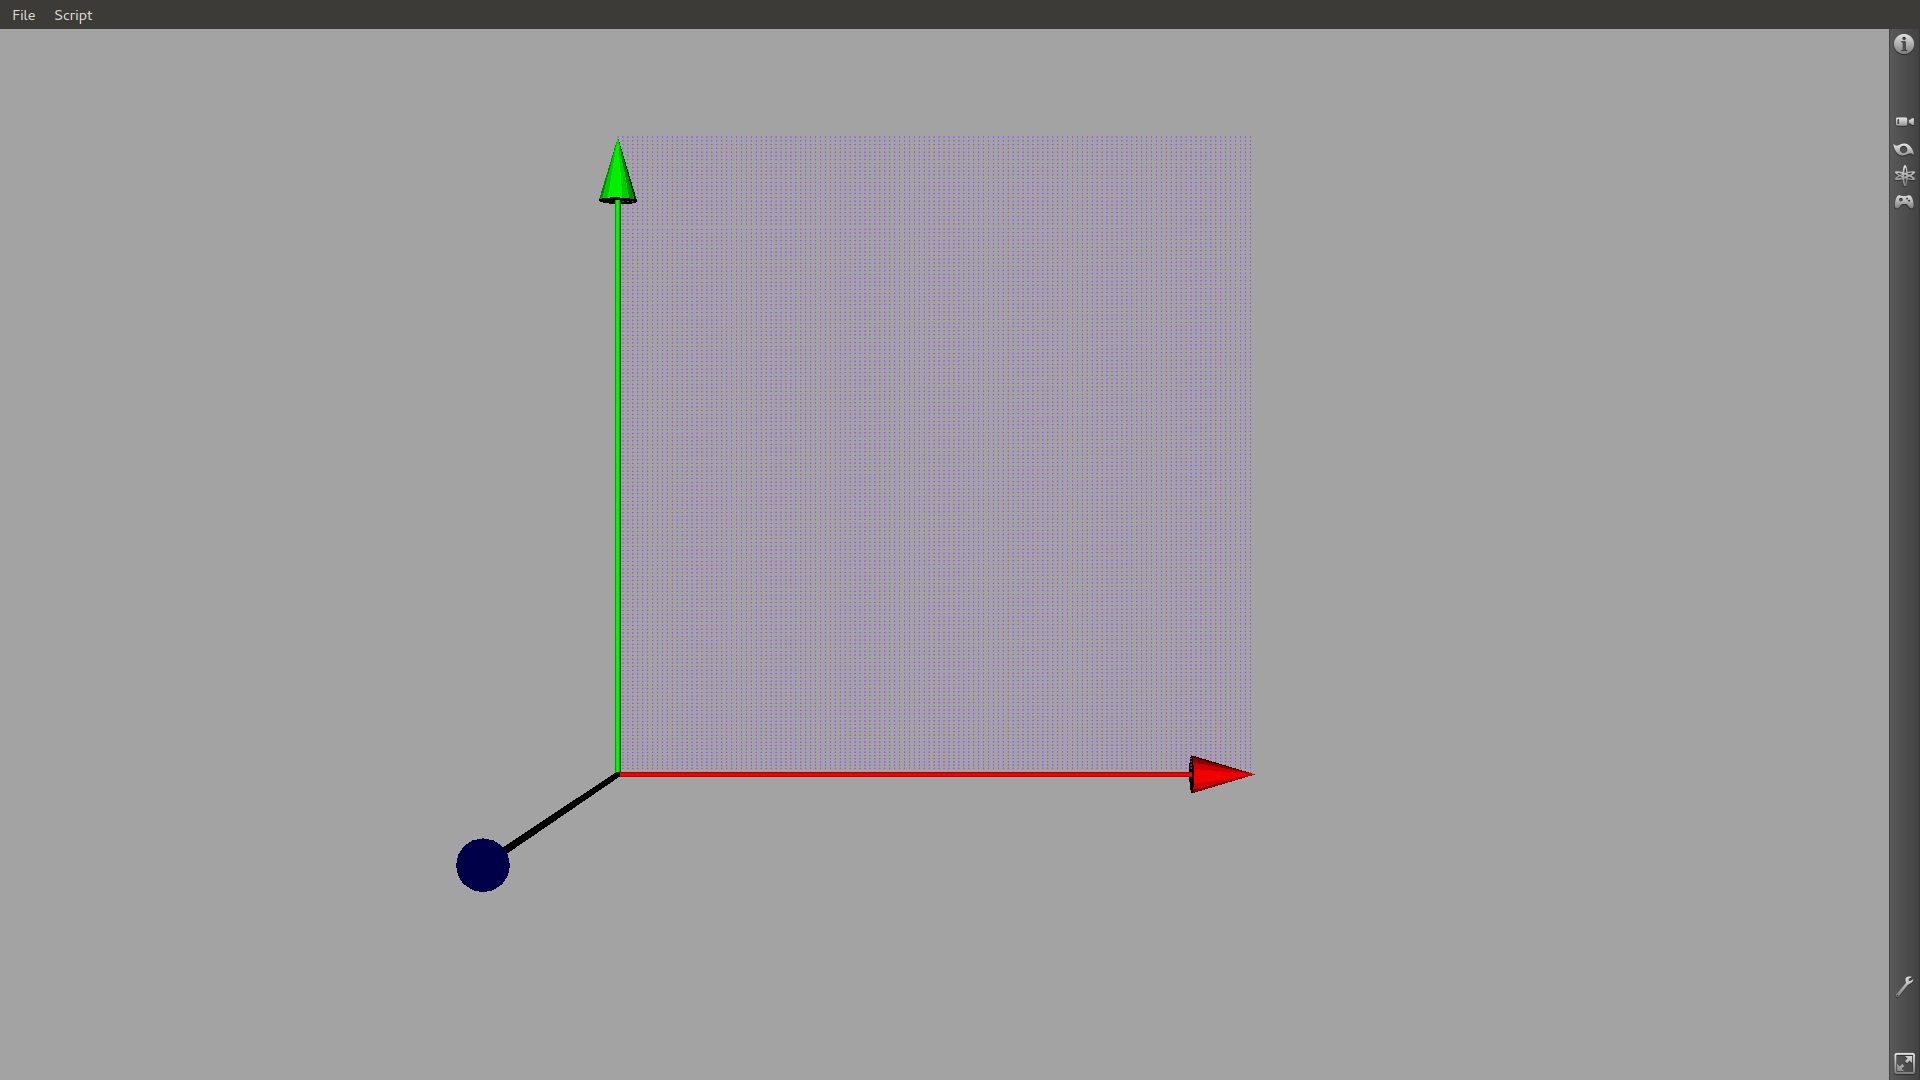
\includegraphics[width=0.5\textwidth]{PICTURES2/parameter_logarithmic.png}\label{fig:f2}}
  \caption{Parametric mesh before(a) and  after(b) logarithmic transformation}
\end{figure}




 


 

\begin{lstlisting}[label=some-code,breaklines=true,caption=fitting process]
#ifndef GET_SURFACE_HPP
#define GET_SURFACE_HPP
#include <axlCore/axlAbstractSurfaceBSpline.h>
#include <axlCore/axlMesh.h>


axlAbstractSurfaceBSpline* get_surface(axlMesh* physical_mesh, axlMesh* parameter_mesh)

{  int rfnmt_loops=4;


    BsplineBasis2D basis_for_mesh(60,40);
    static SplineSurface  *fitted_surface=new SplineSurface;
    double* err_new=new double;
    *err_new=1.e-9;
    SplineSurface *presurf=new SplineSurface;
    presurf=NULL;
    int error_method=0;//SDM
    int opt_method=0; //EDGES FIT=1|GLOBAL_OPT=0
    double lambda=1.e-2;

    RowVectorXd* curve_vector=new RowVectorXd;

    RowVectorXd* error_vector=new RowVectorXd(physical_mesh->vertex_count());
    error_vector->setZero();
    fitted_surface=fitting<axlMesh,axlMesh,BsplineBasis2D>::compute_fit_surf(physical_mesh,parameter_mesh,basis_for_mesh,presurf,error_method,opt_method,lambda,err_new,error_vector,curve_vector,rfnmt_loops);

    axlAbstractSurfaceBSpline* output=new axlAbstractSurfaceBSpline;
    output=dynamic_cast<axlAbstractSurfaceBSpline*>(dtkAbstractDataFactory::instance()->create("goSurfaceBSpline"));
    SplineSurface* tmp  = static_cast<SplineSurface *>(output->surface());
    *tmp = *fitted_surface;
    return output;
}

#endif // GET_SURFACE_HPP


\end{lstlisting}


\newpage
\section{Generating surface between bodies}
Let $d(\tau)$ represent the curve describing a different air foil curve.The same properties described above between the two air foil bodies must apply as well.Using  the subdivision described above we proceed by introducing a new subdivision algorithm(\textbf{{get\_meshes.hpp}},\textbf{get\_meshes\_body(...)} ) this time taking place along the line segments $P_{i}X_{i}$,$P_{i} \in s(t)$,$X_{i} \in d(\tau)$ which calculates new points(\textbf{\textit{Listing 7,Line 39}}): $$Q_{ij}^{n}=\frac{Q_{ij-1}^{n-1}+Q_{ij}^{n-1}}{2}$$

where $Q_{ij-1}^{n-1},Q_{ij}^{n-1} \in P_{i}X_{i}$, $Q_{ij-1}^{0}\equiv P_i$ and $Q_{ij}^{0}\equiv X_i$.

If $(u_{i},v_{i}) \in \widehat{\Omega} $  represent the parametric coordinates of the air foil then the new subdivision algorithm functions  under the criteria(\textbf{\textit{Listing 7,Line 37}}):

\begin{frame}

\begin{minipage}{.45\linewidth}
\begin{center}

\begin{algorithm}[H]


\eIf{\small
$\vert u_{i}^{n-1} - u_{i-1}^{n-1} \vert \geq \frac{1}{M_{0}}$
}{
proceed Subdivision\;
}{
Stop\;
}
\end{algorithm}

\end{center}
\end{minipage}
\end{frame}

\begin{lstlisting}[label=some-code,breaklines=true,caption=Subdivision Algorithm]
void get_meshes_body(  axlAbstractCurveBSpline* axlcurve, axlAbstractCurveBSpline*  contour_curve,axlMesh* physical_mesh,axlMesh* parameter_mesh, double points_on_line, double points_on_curve)
{...
for (int i=0;i<P.size();i++)

    {
        std::vector<double> v;
        std::vector<axlPoint> Q;
        axlPoint    Q_start=P.at(i);
        Q.push_back(Q_start);
        u.push_back(0);
        axlPoint     Q_finish=contour_curve->eval(step);
        Q.push_back(Q_finish);
        u.push_back(1);
      

        std::map<int,int> edge;
        edge[0]=1;
        int b,e;
        std::list<int> stack;
        stack.push_front(0);
        count=2;
        distfield_curve<axlAbstractCurveBSpline>* dst=new  distfield_curve<axlAbstractCurveBSpline> (axlcurve,100000);
        while(!stack.empty())
        {

            std::list<int>::iterator it=stack.begin();
            b=*it;
            stack.pop_front();
            e=edge[b];
            axlPoint Q_b=Q.at(b);
            axlPoint  Q_e=Q.at(e);
            double v_b=v.at(b);
            double v_e=v.at(e);



            if(fabs(v_b-v_e)>1/points_on_line)
            {
                axlPoint Q_middle_on_line=(Q.at(b)+Q.at(e))/2;
                double v_middle=v_value(Q_middle_on_line,Q_start,Q_finish,dst,points_on_line);
                v.push_back(v_middle);
                Q.push_back(Q_middle_on_line);


                int n=Q.size()-1;
                edge[b]=n;
                edge[n]=e;
                stack.push_back(b);
                stack.push_back(n);

                count++;

            }
          
    ...    }
\end{lstlisting}


This times we are calculating the parameter domain coordinate $v_{i}$ which serves as well as the stopping criteria for subdivision.
Let $$v_{i_{0}}=(1-\theta)\Vert \frac{Q_{ij}^{n}P_{i}}{Q_{ij}^{n}X_{i}} \Vert + \theta Q_{ij}^{n}P_{i}$$

where: \\
$$\theta=\begin{cases}1, if \;\Vert Q_{ij}^{n} P_{i}\Vert<d_{0} \\
 2d_{0} - \frac{ \Vert Q_{ij}^{n} P_{i} \Vert}{ d_{0} }, if \; \Vert Q_{ij}^{n} P_{i}\Vert <2d_{0}\\
 0 , else \end{cases}$$
 
 
 The points $ v_{i_{o}} $remain the same or submitted to a logarithmic transform depending on $d_{0}$ thus obtaining the parametric coordinates $v_{i}$(\textbf{\textit{Listing 7,Lines 30-39}}) ,while $u_{i}=i/N$ as in the previous case.
 
 
  
 \begin{figure}
 \begin{center}
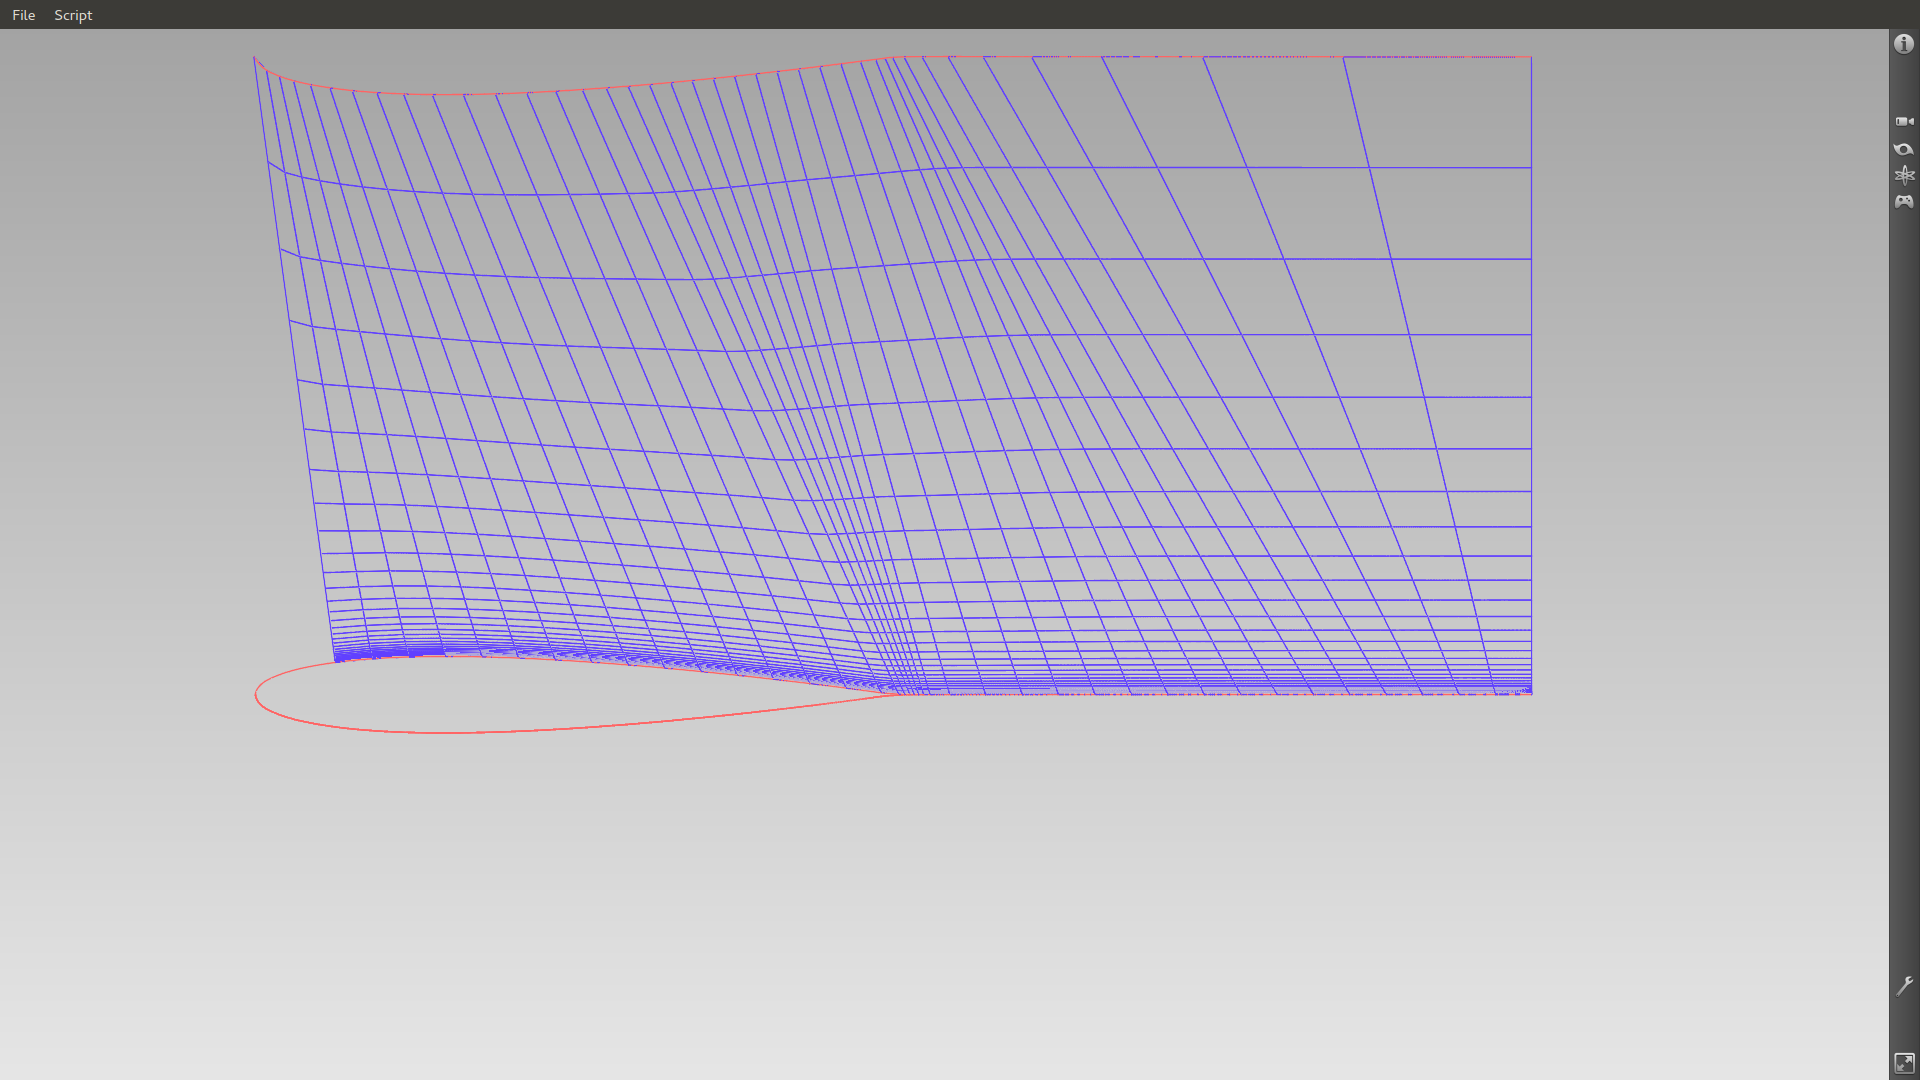
\includegraphics[scale=0.2]{PICTURES2/Other_body_surface.png} 
\end{center}
\caption{Surface generated between two air foils}
 \end{figure}

 
\begin{lstlisting}[label=some-code,breaklines=true,caption=Subdivision Criteria]
double v_value(const axlPoint &Q,const axlPoint &P,const axlPoint &X,distfield_curve<axlAbstractCurveBSpline>* dst,const double  &points_on_line)
{
    double r=1.1;
    double a=pow(r,points_on_line-1);
    double d0=1;

    double b=d0/(pow(a,d0)-1);



    double distance_Q=dst->distance(Q.x(),Q.y(),Q.z());
    double barycentric_Q=axlPoint::distance(Q,P)/axlPoint::distance(P,X);
    double theta,v0,v;

    if(distance_Q<d0)
    {
        theta=1;
    }
    else if(distance_Q>2*d0)
    {
        theta=0;
    }
    else
    {
        theta=2-(distance_Q/d0);
    }
    theta=0;
    v0=(1-theta)*barycentric_Q+distance_Q*theta;

    if (v0<=d0)
    {
        v=(log(v0+b)-log(b))/log(a);
    }
    else
    {
        v=v0;

    }
    return v;

}

}
\end{lstlisting}





\end{document}
